\documentclass[twoside]{article}
\usepackage{graphics}
\usepackage{listings}
\usepackage{amsfonts}
\usepackage{graphicx}
\graphicspath{ {./} }
\usepackage{amsmath}
\usepackage{amssymb}

\setlength{\oddsidemargin}{0.25 in}
\setlength{\evensidemargin}{-0.25 in}
\setlength{\topmargin}{-0.6 in}
\setlength{\textwidth}{6.5 in}
\setlength{\textheight}{8.5 in}
\setlength{\headsep}{0.75 in}
\setlength{\parindent}{0 in}
\setlength{\parskip}{0.1 in}

%
% The following commands set up the lecnum (lecture number)
% counter and make various numbering schemes work relative
% to the lecture number.
%
\newcounter{lecnum}
\renewcommand{\thepage}{\thelecnum-\arabic{page}}
\renewcommand{\thesection}{\thelecnum.\arabic{section}}
\renewcommand{\theequation}{\thelecnum.\arabic{equation}}
\renewcommand{\thefigure}{\thelecnum.\arabic{figure}}
\renewcommand{\thetable}{\thelecnum.\arabic{table}}

%
% The following macro is used to generate the header.
%
\newcommand{\lecture}[5]{
   \pagestyle{myheadings}
   \thispagestyle{plain}
   \newpage
   \setcounter{lecnum}{#1}
   \setcounter{page}{1}
   \noindent
   \begin{center}
   \framebox{
      \vbox{\vspace{2mm}
    \hbox to 6.28in { {\bf EE 382V: Introduction to Social Computing
                        \hfill Fall 2018} }
       \vspace{4mm}
       \hbox to 6.28in { {\Large \hfill Lecture #1: #2  \hfill} }
       \vspace{2mm}       
       \hbox to 6.28in { {\Large \hfill #5  \hfill} }
       \vspace{2mm}
       \hbox to 6.28in { {\it Lecturer: #3 \hfill Scribe: #4} }
      \vspace{2mm}}
   }
   \end{center}
   \markboth{Lecture #1: #2}{Lecture #1: #2}
   %{\bf Disclaimer}: {\it These notes have not been subjected to the
   %usual scrutiny reserved for formal publications.  They may be distributed
   %outside this class only with the permission of the Instructor.}
   \vspace*{4mm}
}

%
% Convention for citations is authors' initials followed by the year.
% For example, to cite a paper by Leighton and Maggs you would type
% \cite{LM89}, and to cite a paper by Strassen you would type \cite{S69}.
% (To avoid bibliography problems, for now we redefine the \cite command.)
% Also commands that create a suitable format for the reference list.
\renewcommand{\cite}[1]{[#1]}
\def\beginrefs{\begin{list}%
        {[\arabic{equation}]}{\usecounter{equation}
         \setlength{\leftmargin}{2.0truecm}\setlength{\labelsep}{0.4truecm}%
         \setlength{\labelwidth}{1.6truecm}}}
\def\endrefs{\end{list}}
\def\bibentry#1{\item[\hbox{[#1]}]}

%Use this command for a figure; it puts a figure in wherever you want it.
%usage: \fig{NUMBER}{SPACE-IN-INCHES}{CAPTION}
\newcommand{\fig}[3]{
			\vspace{#2}
			\begin{center}
			Figure \thelecnum.#1:~#3
			\end{center}
	}
% Use these for theorems, lemmas, proofs, etc.
\newtheorem{theorem}{Theorem}[lecnum]
\newtheorem{lemma}[theorem]{Lemma}
\newtheorem{proposition}[theorem]{Proposition}
\newtheorem{claim}[theorem]{Claim}
\newtheorem{corollary}[theorem]{Corollary}
\newtheorem{definition}[theorem]{Definition}
\newenvironment{proof}{{\bf Proof:}}{\hfill\rule{2mm}{2mm}}

% **** IF YOU WANT TO DEFINE ADDITIONAL MACROS FOR YOURSELF, PUT THEM HERE:

\begin{document}
%FILL IN THE RIGHT INFO.
\lecture{4 Session 1}{September 29}{Vijay Garg}{Tiffany Tillett}{Stable Marriage}
%\footnotetext{These notes are partially based on those of Nigel Mansell.}

% **** YOUR NOTES GO HERE:

% Some general latex examples and examples making use of the
% macros follow.  
%**** IN GENERAL, BE BRIEF. LONG SCRIBE NOTES, NO MATTER HOW WELL WRITTEN,
%**** ARE NEVER READ BY ANYBODY.
\section{Review}

Recall the algorithm to find a stable marriage from last class.

\subsection{Inputs}
\begin{enumerate}
    \item mPref: data structure containing preferences for each man
    \item wPref: data structure containing preferences for each woman
    \item rank: where rank[i][j] indicates the rank of man j for woman i; higher preference correlates to lower rank
\end{enumerate}

\subsection{Stable Marriage Algorithm}
\begin{enumerate}
    \item $freelist$ = list of men who are free (initially has all men)
    \item while ($freelist$ is not empty):
    {\setlength\itemindent{25pt} \item choose some man $m$ from $freelist$}
    {\setlength\itemindent{25pt} \item $m$ proposes to his most preferred woman $w$ that he has not already proposed to}
    {\setlength\itemindent{25pt} \item if $w$ is free:}
    {\setlength\itemindent{50pt} \item $w$ accepts proposal (assign $m$ to $w$)}
    {\setlength\itemindent{25pt} \item else: // $w$ is already engaged to $m'$}
    {\setlength\itemindent{50pt} \item if $rank[w][m] > rank[w][m']$: // $w$ prefers $m'$}
    {\setlength\itemindent{75pt} \item add $m$ back to $freelist$ // reject $m$; $w$ still engaged to $m'$}
    {\setlength\itemindent{50pt} \item else:}
    {\setlength\itemindent{75pt} \item add $m'$ back to the $freelist$ // reject $m'$}
    {\setlength\itemindent{75pt} \item $w$ gets engaged to $m$}
    \item print assignment
    
\end{enumerate}

\section{Stable Marriage Algorithm Correctness}

\begin{theorem}
The Algorithm terminates with a matching.
\end{theorem}

\begin{proof}

\begin{claim}
The last woman in a man's preference list must be free
\end{claim}


Invariant: Once a woman is engaged, she stays engaged.

In order for a man to make it to his last preference, the previous $n-1$ women must already be engaged since the only reason they can reject his proposal is if they are engaged to someone that they prefer more. Since the number of men and women is equal, the last woman in the list can never be engaged.

Since the last woman in a man's preference list will always be free, every man is guaranteed that he will match with one woman, so a matching will exist.

\end{proof}

\begin{theorem}
The algorithm (if it terminates) ends with a stable matching.
\end{theorem}

\begin{proof}
Assume that $(m,w')(m',w)$ is a blocking pair where $m$ is married to $w'$ and $w$ is married to $m'$.

In order for $(m,w')(m',w)$ to be a blocking pair, this means that $m$ must prefer $w$ to $w'$ and that $w$ must prefer $m$ to $m'$.

Since $m$ prefers $w$ to $w'$, he would have proposed to $w$ first and gotten rejected.

Invariant: A woman's assignment can only improve with execution of the algorithm.

Therefore, $w$ can only have rejected $m$ if she had a proposal from someone she preferred more. If that person was $m'$, we know that she must prefer $m'$ to $m$. If that person was not $m'$, we know that she prefers that person to $m$ and that she prefers $m'$ to that person, so by extension, she prefers $m'$ to $m$. Generally, $w$ will always prefer her current fiance to all men she rejected, so she must prefer $m'$ to $m$. 

The requirement for $(m,w)$ to be a blocking pair was that $m$ must prefer $w$ to $w'$ and that $w$ must prefer $m$ to $m'$. These two requirements cannot co-exist, so by contradiction, we know that $(m,w')(m',w)$ cannot be a blocking pair.
\end{proof}

\section{Posets: Partially Ordered Sets}

\subsection{Definition}
A poset is defined as $(X, \leq)$ where $X$ is a set and $\leq$ is a binary relation on that set.

A reflexive poset has the following properties:
\begin{enumerate}
    \item reflexive - for all vertices $v$ in $V$: $v \leq v$
    \item anti-symmetric - for all pairs of vertices $u,v$ in $V$: if $v \leq u$ and $u \leq v$ then $u == v$
    \item transitive - for all groups of vertices $u,v,w$ in $V$: $u \leq v \leq w$ implies that $u \leq w$
\end{enumerate}

Consider all following posets to be reflexive posets.

\subsection{Example 1}
$X$: $\mathbb{R}^n$

$\leq$: $U \leq V$ $\equiv$ for all i: $u[i] \leq v[i]$

\begin{claim}
$(X, \leq)$ is a poset.
\end{claim}

\subsubsection{Numerical Example 1}
$M1 = (2,5,3)$; $M2 = (6,8,5)$

$2 \leq 6$, $5 \leq 8$, $3 \leq 5$ says that $M1 \leq M2$.

\subsubsection{Numerical Example 2}
$M1 = (1,3,1)$; $M2 = (2,1,2)$

$1 \leq 2$, $3 > 1$. What does this mean?

\begin{definition}
$M1$ is incomparable to $M2$ if $(M1 \nleq M2)$ and $(M2 \nleq M1)$.
\end{definition}

\vspace{3mm} %5mm vertical space

\subsection{Example 2}
$z = \{a, b, c\}$

$X$: \{ \{\}, \{a\}, \{b\}, \{c\}, \{a,b\}, \{a,c\}, \{b,c\}, \{a,b,c\} \}

$\leq$: $\subseteq$
\newline

$\{a,b\} \leq \{a,b,c\}$

$\{a,b\}$ is incomparable to $\{b,c\}$

\subsection{Dealing with Incomparable Items}
If $M1$ and $M2$ are incomparable, try to find $M3$ which is better than both $M1$ and $M2$.
\newline

$M1 = (1,1,2,3)$

$M2 = (2,2,1,2)$

Note: the numbers here indicate preference where 1 indicates first choice, 2 indicates second choice, etc
\newline

find $M3 = (1,1,1,2)$ such that $M3 \leq M1$ and $M3 \leq M2$.

\subsection{Hasse Diagrams: Pictoral Representations of Posets}
\begin{figure}[h]
\centering
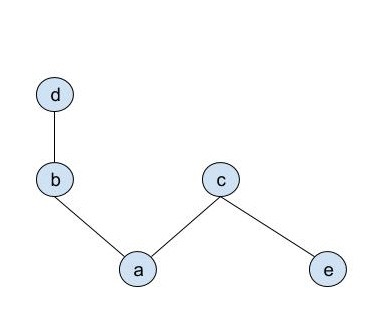
\includegraphics[width=.8\textwidth]{hasse.jpg}
\end{figure}
\fig{1}{0cm}{Hasse Diagram example}

This diagram shows that:

$a \leq b$

$a \leq c$

$b \leq d$

$e \leq c$

$c$ and $d$ are incomparable

$a$ and $e$ are incomparable

\subsection{Operations on Posets}
Given a poset $(X, \leq)$:


\begin{definition}
Let $x,y \in X$. $z \in X$ is meet of $x$ and $y$ if:
\begin{enumerate}
    \item $z \leq x$ and $z \leq y$    
    
    AND
    \item for all $z'$: $z' \leq x$ and $z' \leq y \implies z' \leq z$
\end{enumerate}

Where meet is also known as the greatest lower bound. The first condition is the lower bound, and the second condition is that the lower bound must be greater than all other lower bounds.
\end{definition} 

\begin{minipage}[]{\textwidth}
\centering
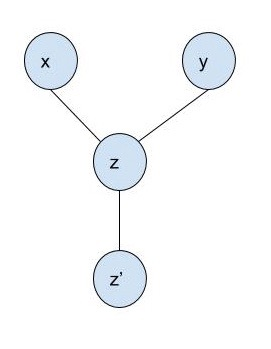
\includegraphics[width=.5\textwidth]{meet.jpg}
\end{minipage}
\fig{2}{0cm}{Meet Example; z is the meet of x and y}

\begin{minipage}[]{\textwidth}
\centering
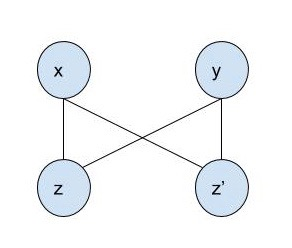
\includegraphics[width=.5\textwidth]{incomparable.jpg}
\end{minipage}
\fig{3}{0cm}{z is not a meet; z and z' are incomparable}

\begin{minipage}[]{\textwidth}
\centering
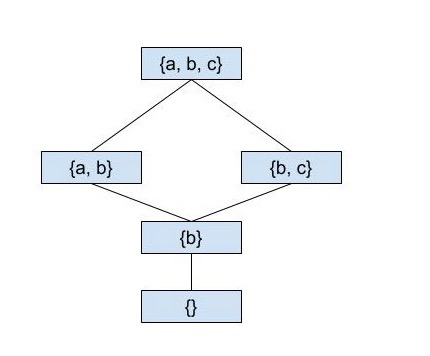
\includegraphics[width=.5\textwidth]{meet_intersection.jpg}
\end{minipage}
\fig{4}{0cm}{meet corresponds to intersection of sets}

\subsection{Lattice Posets}
\begin{definition}
A poset $(X, \leq)$ is lattice (nice) if for all $a,b \in X$, $meet(a, b)$ exists and $join(a,b)$ exists.
\end{definition}

\begin{definition}
$join(a,b)$ is the greatest lower bound (reverse of meet).
\end{definition}

$(a \vee b)$ = $join(a,b)$

$(a \wedge b)$ = $meet(a,b)$


\begin{minipage}[]{\textwidth}
\centering
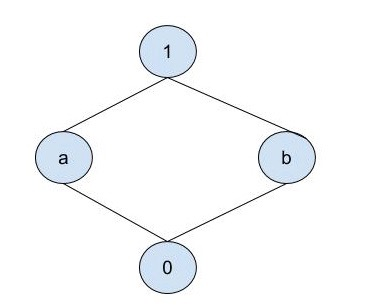
\includegraphics[width=.5\textwidth]{lattice1.jpg}
\end{minipage}
\fig{5}{0cm}{meet(a,1) = a}

\begin{minipage}[]{\textwidth}
\centering
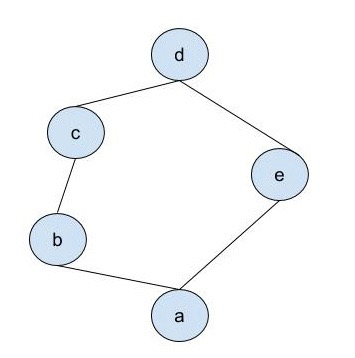
\includegraphics[width=.5\textwidth]{lattice2.jpg}
\end{minipage}
\fig{6}{0cm}{meet(c,e) = a; join(c,e) = d; meet(b,e) = a; join(b,e) = d}

\begin{minipage}[]{\textwidth}
\centering
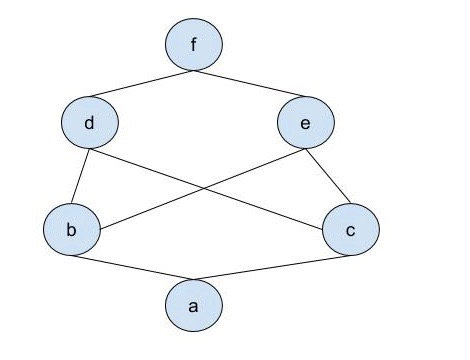
\includegraphics[width=.5\textwidth]{lattice3.jpg}
\end{minipage}
\fig{7}{0cm}{meet(b,c) = a; There is no meet of $d$ and $e$ since $b$ and $c$ are incomparable. $a$ cannot be the meet since $b$ and $c$ are bigger than $a$.}

The definition of a lattice can be extended to apply to all finite subsets of $X$.

\begin{definition}
A lattice $L = (X, \leq$ is distributive if for all $x,y,z \in X$: 
\begin{enumerate}
    \item $x \wedge (y \vee z) = (x \wedge y) \vee (x \wedge z)$
    
    OR
    
    \item $x \vee (y \wedge z) = (x \vee y) \wedge (x \vee z)$
\end{enumerate}
\end{definition}
\vspace{.5cm}

Referencing Figure 11.6:

$e \wedge (b \vee c) = e \wedge c = a$

$(e \wedge b) \vee (e \wedge c) = a \vee a = a$

\vspace{.2cm}
This works out. However, we need to show this for all $x,y,z$.

\vspace{.2cm}
$c \wedge (b \vee e) = c \wedge d = c$

$(c \wedge b) \vee (c \wedge e) = b \vee a = b$.

\vspace{.2cm}
This does not work. This lattice is not distributive.
\vspace{.2cm}

There is a theorem which states that lattices of certain shapes cannot be distributive.


\end{document}





